\documentclass{beamer}
\usetheme{Madrid}
\usecolortheme{default}

\usepackage{listings}
\usepackage{xcolor}
\usepackage{algorithmic}
\usepackage{tikz}

% Listing settings
\lstset{
    basicstyle=\ttfamily\footnotesize,
    keywordstyle=\color{blue},
    commentstyle=\color{green!50!black},
    stringstyle=\color{red},
    showstringspaces=false,
    breaklines=true,
    frame=single
}

\title{The Reader-Writer Problem}
\subtitle{Implementation and Analysis of Synchronization Strategies}
\author{Your Name}
\institute{Your University}
\date{\today}

\begin{document}

% Title Slide
\begin{frame}
\titlepage
\end{frame}

% Table of Contents
\begin{frame}{Outline}
\tableofcontents
\end{frame}

% Section 1: Introduction
\section{Introduction}

\begin{frame}{The Reader-Writer Problem}
\begin{block}{Problem Statement}
Multiple concurrent threads accessing shared resources:
\begin{itemize}
    \item \textbf{Readers}: Only read data (can operate concurrently)
    \item \textbf{Writers}: Modify data (require exclusive access)
\end{itemize}
\end{block}

\vspace{0.5cm}

\begin{block}{Challenge}
Allow multiple readers \textbf{OR} one writer at a time, while maintaining:
\begin{itemize}
    \item \textbf{Correctness}: No data corruption
    \item \textbf{Performance}: Maximize throughput
    \item \textbf{Fairness}: Prevent starvation
\end{itemize}
\end{block}
\end{frame}

\begin{frame}{Real-World Applications}
\begin{columns}
\column{0.5\textwidth}
\textbf{Database Systems}
\begin{itemize}
    \item PostgreSQL
    \item MySQL InnoDB
    \item Read/Write transactions
\end{itemize}

\vspace{0.3cm}

\textbf{Operating Systems}
\begin{itemize}
    \item Linux kernel RW semaphores
    \item File system access
    \item Process synchronization
\end{itemize}

\column{0.5\textwidth}
\textbf{Programming Languages}
\begin{itemize}
    \item Java ReadWriteLock
    \item C++ shared\_mutex
    \item Rust RwLock
\end{itemize}

\vspace{0.3cm}

\textbf{Distributed Systems}
\begin{itemize}
    \item Cache coherence
    \item Shared memory
    \item Configuration services
\end{itemize}
\end{columns}
\end{frame}

\begin{frame}{Research Contributions}
\begin{enumerate}
    \item \textbf{Unified Framework}: Single API supporting 4 synchronization modes
    \vspace{0.2cm}
    
    \item \textbf{Comprehensive Testing}: 16 automated runs demonstrating race conditions and correctness
    \vspace{0.2cm}
    
    \item \textbf{Quantitative Analysis}: Performance trade-offs between strategies
    \vspace{0.2cm}
    
    \item \textbf{Practical Insights}: Implementation guidance for real systems
\end{enumerate}
\end{frame}

% Section 2: Architecture
\section{System Architecture}

\begin{frame}{Three-Layer Architecture}
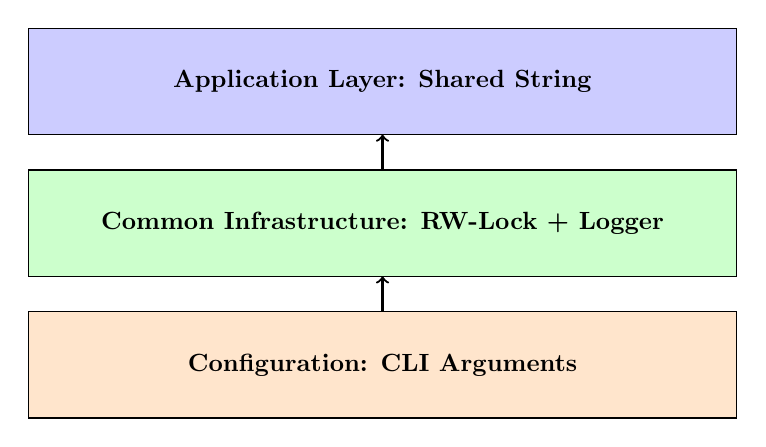
\begin{tikzpicture}[scale=0.9, every node/.style={scale=0.9}]
    % Layer 3 - Application
    \draw[fill=blue!20] (0,6) rectangle (10,7.5);
    \node at (5,6.75) {\textbf{Application Layer: Shared String}};
    
    % Layer 2 - Infrastructure
    \draw[fill=green!20] (0,4) rectangle (10,5.5);
    \node at (5,4.75) {\textbf{Common Infrastructure: RW-Lock + Logger}};
    
    % Layer 1 - Foundation
    \draw[fill=orange!20] (0,2) rectangle (10,3.5);
    \node at (5,2.75) {\textbf{Configuration: CLI Arguments}};
    
    % Arrows
    \draw[->,thick] (5,5.5) -- (5,6);
    \draw[->,thick] (5,3.5) -- (5,4);
\end{tikzpicture}

\vspace{0.3cm}

\textbf{Benefits:}
\begin{itemize}
    \item Easy mode comparison (single parameter change)
    \item Reusable synchronization primitives
    \item Configurable test scenarios
\end{itemize}
\end{frame}

\begin{frame}[fragile]{Unified Lock API}
\begin{lstlisting}[language=C]
typedef enum {
    VANILLA,      // No synchronization
    READER_PREF,  // Reader preference
    WRITER_PREF,  // Writer preference
    FAIR          // Fair scheduling
} rw_mode_t;

// Unified API
void rw_init(rw_lock_t *lock, rw_mode_t mode);
void reader_enter(rw_lock_t *lock);
void reader_exit(rw_lock_t *lock);
void writer_enter(rw_lock_t *lock);
void writer_exit(rw_lock_t *lock);
void rw_destroy(rw_lock_t *lock);
\end{lstlisting}

\textbf{Key advantage}: Performance differences purely due to synchronization strategy, not implementation variations
\end{frame}

\begin{frame}{Synchronization Primitives}
\begin{block}{Mutex-Based Implementation (Our Choice)}
\begin{itemize}
    \item Uses \texttt{pthread\_mutex\_t}
    \item Better integration with condition variables
    \item Clearer ownership semantics
    \item Widely supported in POSIX
\end{itemize}
\end{block}

\vspace{0.3cm}

\begin{block}{Alternative: Semaphore-Based}
\begin{itemize}
    \item Uses counting semaphores
    \item Simpler conceptual model for some algorithms
    \item Common in textbook solutions
\end{itemize}
\end{block}

\vspace{0.2cm}
\textbf{Note}: Both approaches are equally valid. Reader/Writer Preference and Fair scheduling are \textbf{algorithms}, not primitives.
\end{frame}

% Section 3: Implementation
\section{Implementation}

\begin{frame}{Shared String Application}
\begin{block}{Shared Resource}
\texttt{char shared\_string[256]} - A mutable string buffer
\end{block}

\vspace{0.3cm}

\begin{columns}
\column{0.5\textwidth}
\textbf{Writer Behavior:}
\begin{enumerate}
    \item Select sentence from 20 predefined strings
    \item Acquire writer lock
    \item Copy sentence character-by-character
    \item Release lock
    \item Log operation
\end{enumerate}

\column{0.5\textwidth}
\textbf{Reader Behavior:}
\begin{enumerate}
    \item Acquire reader lock
    \item Read entire string
    \item Release lock
    \item Validate against valid set
    \item Log operation
\end{enumerate}
\end{columns}

\vspace{0.3cm}
\begin{alertblock}{Race Condition: Torn Reads}
Without synchronization, readers see partial updates: \\
\texttt{"Syncating systems manage..."} (mixed sentences)
\end{alertblock}
\end{frame}

% Section 4: Synchronization Modes
\section{Synchronization Modes}

\begin{frame}[fragile]{Mode 1: Vanilla (No Synchronization)}
\begin{lstlisting}[language=C]
void reader_enter(rw_lock_t *lock) {
    // No synchronization!
    lock->active_readers++;
}
\end{lstlisting}

\vspace{0.3cm}

\begin{block}{Purpose}
Baseline to demonstrate race conditions
\end{block}

\vspace{0.3cm}

\begin{alertblock}{Expected Behavior}
\begin{itemize}
    \item Data corruption (torn reads)
    \item Lost updates
    \item \textbf{DO NOT USE IN PRODUCTION!}
\end{itemize}
\end{alertblock}
\end{frame}

\begin{frame}{Mode 2: Reader Preference}
\begin{block}{Algorithm}
\begin{itemize}
    \item First reader locks resource
    \item Subsequent readers increment counter (no blocking)
    \item Last reader unlocks resource
    \item Writers wait for all readers to finish
\end{itemize}
\end{block}

\vspace{0.3cm}

\begin{columns}
\column{0.5\textwidth}
\textbf{Advantages:}
\begin{itemize}
    \item Maximizes read throughput
    \item Multiple concurrent readers
    \item Low reader latency
\end{itemize}

\column{0.5\textwidth}
\textbf{Disadvantages:}
\begin{itemize}
    \item \alert{Writer starvation}
    \item Continuous readers block writers indefinitely
\end{itemize}
\end{columns}

\vspace{0.3cm}
\textbf{Use case}: Read-heavy workloads with infrequent writes
\end{frame}

\begin{frame}{Mode 3: Writer Preference}
\begin{block}{Algorithm}
\begin{itemize}
    \item Writers acquire \texttt{read\_try} lock
    \item Blocks new readers when writers waiting
    \item Existing readers finish, then writer executes
    \item Readers wait for all writers to complete
\end{itemize}
\end{block}

\vspace{0.3cm}

\begin{columns}
\column{0.5\textwidth}
\textbf{Advantages:}
\begin{itemize}
    \item Prevents writer starvation
    \item Ensures timely updates
    \item Data freshness
\end{itemize}

\column{0.5\textwidth}
\textbf{Disadvantages:}
\begin{itemize}
    \item \alert{Reader starvation}
    \item Continuous writers delay readers
\end{itemize}
\end{columns}

\vspace{0.3cm}
\textbf{Use case}: Write-heavy workloads requiring fresh data
\end{frame}

\begin{frame}{Mode 4: Fair Scheduling (Turnstile Pattern)}
\begin{block}{Algorithm}
\begin{itemize}
    \item All threads pass through \texttt{queue\_lock} "turnstile"
    \item FIFO ordering - no cutting in line
    \item Both readers and writers get fair access
    \item Prevents starvation of either type
\end{itemize}
\end{block}

\vspace{0.3cm}

\begin{columns}
\column{0.5\textwidth}
\textbf{Advantages:}
\begin{itemize}
    \item \textcolor{green!50!black}{No starvation}
    \item Balanced access
    \item Predictable latency
\end{itemize}

\column{0.5\textwidth}
\textbf{Disadvantages:}
\begin{itemize}
    \item Slight throughput reduction
    \item Extra lock overhead
\end{itemize}
\end{columns}

\vspace{0.3cm}
\textbf{Use case}: Mixed workloads requiring fairness guarantees
\end{frame}

\begin{frame}{Comparison Summary}
\begin{table}
\centering
\small
\begin{tabular}{|l|c|c|c|}
\hline
\textbf{Mode} & \textbf{Correctness} & \textbf{Starvation} & \textbf{Throughput} \\ \hline
Vanilla & \alert{\textbf{NO}} & N/A & High \\ \hline
Reader Pref & \textcolor{green!50!black}{YES} & Writers & Highest \\ \hline
Writer Pref & \textcolor{green!50!black}{YES} & Readers & Medium \\ \hline
Fair & \textcolor{green!50!black}{YES} & \textcolor{green!50!black}{None} & Medium \\ \hline
\end{tabular}
\end{table}

\vspace{0.5cm}

\textbf{Key Insight}: No single "best" solution - choice depends on:
\begin{itemize}
    \item Workload characteristics (read/write ratio)
    \item Latency requirements
    \item Fairness constraints
\end{itemize}
\end{frame}

% Section 5: Experimental Results
\section{Experimental Results}

\begin{frame}{Test Methodology}
\begin{block}{Automated Testing Framework}
\begin{itemize}
    \item \textbf{Total runs}: 16 (4 modes × 4 runs)
    \item \textbf{Configuration per run}:
    \begin{itemize}
        \item 8 writer threads
        \item 5 reader threads
        \item 8 seconds duration
    \end{itemize}
    \item \textbf{Validation}: 20 predefined valid sentences
    \item \textbf{Detection}: Torn read = any string not in valid set
\end{itemize}
\end{block}

\vspace{0.3cm}

\begin{block}{Tools}
\begin{itemize}
    \item \texttt{run\_tests.sh}: Execute tests, save timestamped logs
    \item \texttt{analyze\_comprehensive.py}: Parse logs, detect errors, generate report
\end{itemize}
\end{block}
\end{frame}

\begin{frame}{Actual Test Results}
\textbf{Session ID}: 20260113\_004235

\vspace{0.3cm}

\begin{table}
\centering
\begin{tabular}{|l|r|r|}
\hline
\textbf{Mode} & \textbf{Clean Runs} & \textbf{Avg Torn Reads} \\ \hline
vanilla & \alert{0/4} & \alert{367} \\ \hline
reader\_pref & \textcolor{green!50!black}{\textbf{4/4}} & \textcolor{green!50!black}{\textbf{0}} \\ \hline
writer\_pref & \textcolor{green!50!black}{\textbf{4/4}} & \textcolor{green!50!black}{\textbf{0}} \\ \hline
fair & \textcolor{green!50!black}{\textbf{4/4}} & \textcolor{green!50!black}{\textbf{0}} \\ \hline
\end{tabular}
\end{table}

\vspace{0.3cm}

\begin{block}{Key Findings}
\begin{itemize}
    \item \textcolor{green!50!black}{\textbf{Perfect validation}}: All synchronized modes 100\% correct (12/12 runs)
    \item \alert{\textbf{Clear problem demonstration}}: Vanilla 0\% success rate
    \item \textbf{No false positives}: Zero errors in synchronized runs
\end{itemize}
\end{block}
\end{frame}

\begin{frame}{Torn Read Examples (Vanilla Mode)}
\begin{exampleblock}{Example Corrupted Strings}
\begin{enumerate}
    \item \texttt{"Syncating systems manage..."}
    \begin{itemize}
        \item Mixed: "Sync" from one sentence + "ating systems" from another
    \end{itemize}
    
    \vspace{0.2cm}
    
    \item \texttt{"Mutal exclusures..."}
    \begin{itemize}
        \item Partial overwrite: "Mutual exclusion" $\rightarrow$ "Mutal exclusures"
    \end{itemize}
    
    \vspace{0.2cm}
    
    \item \texttt{"Pthread libuduce and..."}
    \begin{itemize}
        \item Character-level corruption from race
    \end{itemize}
\end{enumerate}
\end{exampleblock}

\vspace{0.3cm}

\textbf{Average}: 367 torn reads per 8-second vanilla run \\
\textbf{Conclusion}: Concurrent writes without synchronization = severe data corruption
\end{frame}

\begin{frame}{Statistical Significance}
\begin{block}{Test Coverage}
\begin{itemize}
    \item \textbf{16 total runs} across all modes
    \item \textbf{Hundreds of operations} per run (reads + writes)
    \item \textbf{Multiple sessions} with consistent results
\end{itemize}
\end{block}

\vspace{0.3cm}

\begin{block}{Success Rates}
\begin{itemize}
    \item Vanilla: 0/4 clean = \alert{0\% success} (expected)
    \item Synchronized modes: 12/12 clean = \textcolor{green!50!black}{\textbf{100\% success}}
    \item High confidence in implementation correctness
\end{itemize}
\end{block}

\vspace{0.3cm}

\textbf{Reproducibility}: Results consistent across multiple test sessions
\end{frame}

% Section 6: Conclusion
\section{Conclusion}

\begin{frame}{Key Findings}
\begin{enumerate}
    \item \textbf{Vanilla mode demonstrates the problem}
    \begin{itemize}
        \item 100\% race condition rate
        \item Average 367 torn reads per run
        \item Clear evidence of why synchronization is needed
    \end{itemize}
    
    \vspace{0.3cm}
    
    \item \textbf{All synchronized modes achieve correctness}
    \begin{itemize}
        \item 100\% success rate (12/12 runs)
        \item Zero data corruption
        \item Validates implementation
    \end{itemize}
    
    \vspace{0.3cm}
    
    \item \textbf{Trade-offs between strategies}
    \begin{itemize}
        \item Reader preference: High throughput, writer starvation
        \item Writer preference: Data freshness, reader delays
        \item Fair: Balanced, slight overhead
    \end{itemize}
\end{enumerate}
\end{frame}

\begin{frame}{Practical Recommendations}
\begin{block}{When to Use Each Mode}
\textbf{Reader Preference}:
\begin{itemize}
    \item Read-heavy workloads (90\%+ reads)
    \item Infrequent writes acceptable to be delayed
    \item Example: Configuration cache
\end{itemize}

\vspace{0.2cm}

\textbf{Writer Preference}:
\begin{itemize}
    \item Write-heavy workloads
    \item Fresh data critical
    \item Example: Real-time monitoring
\end{itemize}

\vspace{0.2cm}

\textbf{Fair Scheduling}:
\begin{itemize}
    \item Mixed workloads
    \item Fairness guarantees required
    \item Example: Shared services with SLAs
\end{itemize}
\end{block}
\end{frame}

\begin{frame}{Future Directions}
\begin{itemize}
    \item \textbf{Advanced mechanisms}:
    \begin{itemize}
        \item Priority-based scheduling
        \item Adaptive algorithms based on workload
    \end{itemize}
    
    \vspace{0.3cm}
    
    \item \textbf{Lock-free alternatives}:
    \begin{itemize}
        \item Atomic operations
        \item Read-Copy-Update (RCU)
        \item Compare-and-swap patterns
    \end{itemize}
    
    \vspace{0.3cm}
    
    \item \textbf{Performance optimization}:
    \begin{itemize}
        \item NUMA architecture considerations
        \item Cache-line alignment
        \item Fine-grained locking
    \end{itemize}
\end{itemize}
\end{frame}

\begin{frame}{Conclusion}
\begin{block}{Summary}
\begin{itemize}
    \item Implemented and analyzed 4 Reader-Writer synchronization strategies
    \item Demonstrated race conditions and validated correctness through comprehensive testing
    \item Quantified trade-offs between performance, fairness, and starvation
\end{itemize}
\end{block}

\vspace{0.5cm}

\begin{block}{Contributions}
\begin{itemize}
    \item Unified framework for easy comparison
    \item Practical implementation insights
    \item Open-source educational material
\end{itemize}
\end{block}

\vspace{0.5cm}

\centering
\Large{\textbf{Thank You!}}

\vspace{0.3cm}

\normalsize{Questions?}
\end{frame}

\end{document}
